\documentclass{beamer}

\input{./resources/config.tex}
\input{./resources/colors.tex}
%\input{./resources/math.tex}

\begin{document}

\begin{frame}
  \titlepage
\end{frame}

\setcounter{section}{27}
\section{Objekterkennung}

\begin{frame}{Rückblick CNNs}
  \begin{itemize}
    \item Bisher eingesetzt zur Bildklassifikation
    \item Das bedeutet: Das gesamte Bild wird klassifiziert
    \item Somit wird das Bild \textbf{einer} Klasse zugeordnet
    \item []
    \item<2-> Super für Datensätze wie
      \begin{itemize}
        \item \textit{ImageNet}~(siehe~Abb.~\ref{fig:imagenet}),
        \item \textit{GTSRB}~(siehe~Abb.~\ref{fig:gtsrb})
        \item \ldots
      \end{itemize}
  \end{itemize}
\end{frame}

\begin{frame}{ImageNet}
  \begin{figure}
    \centering
    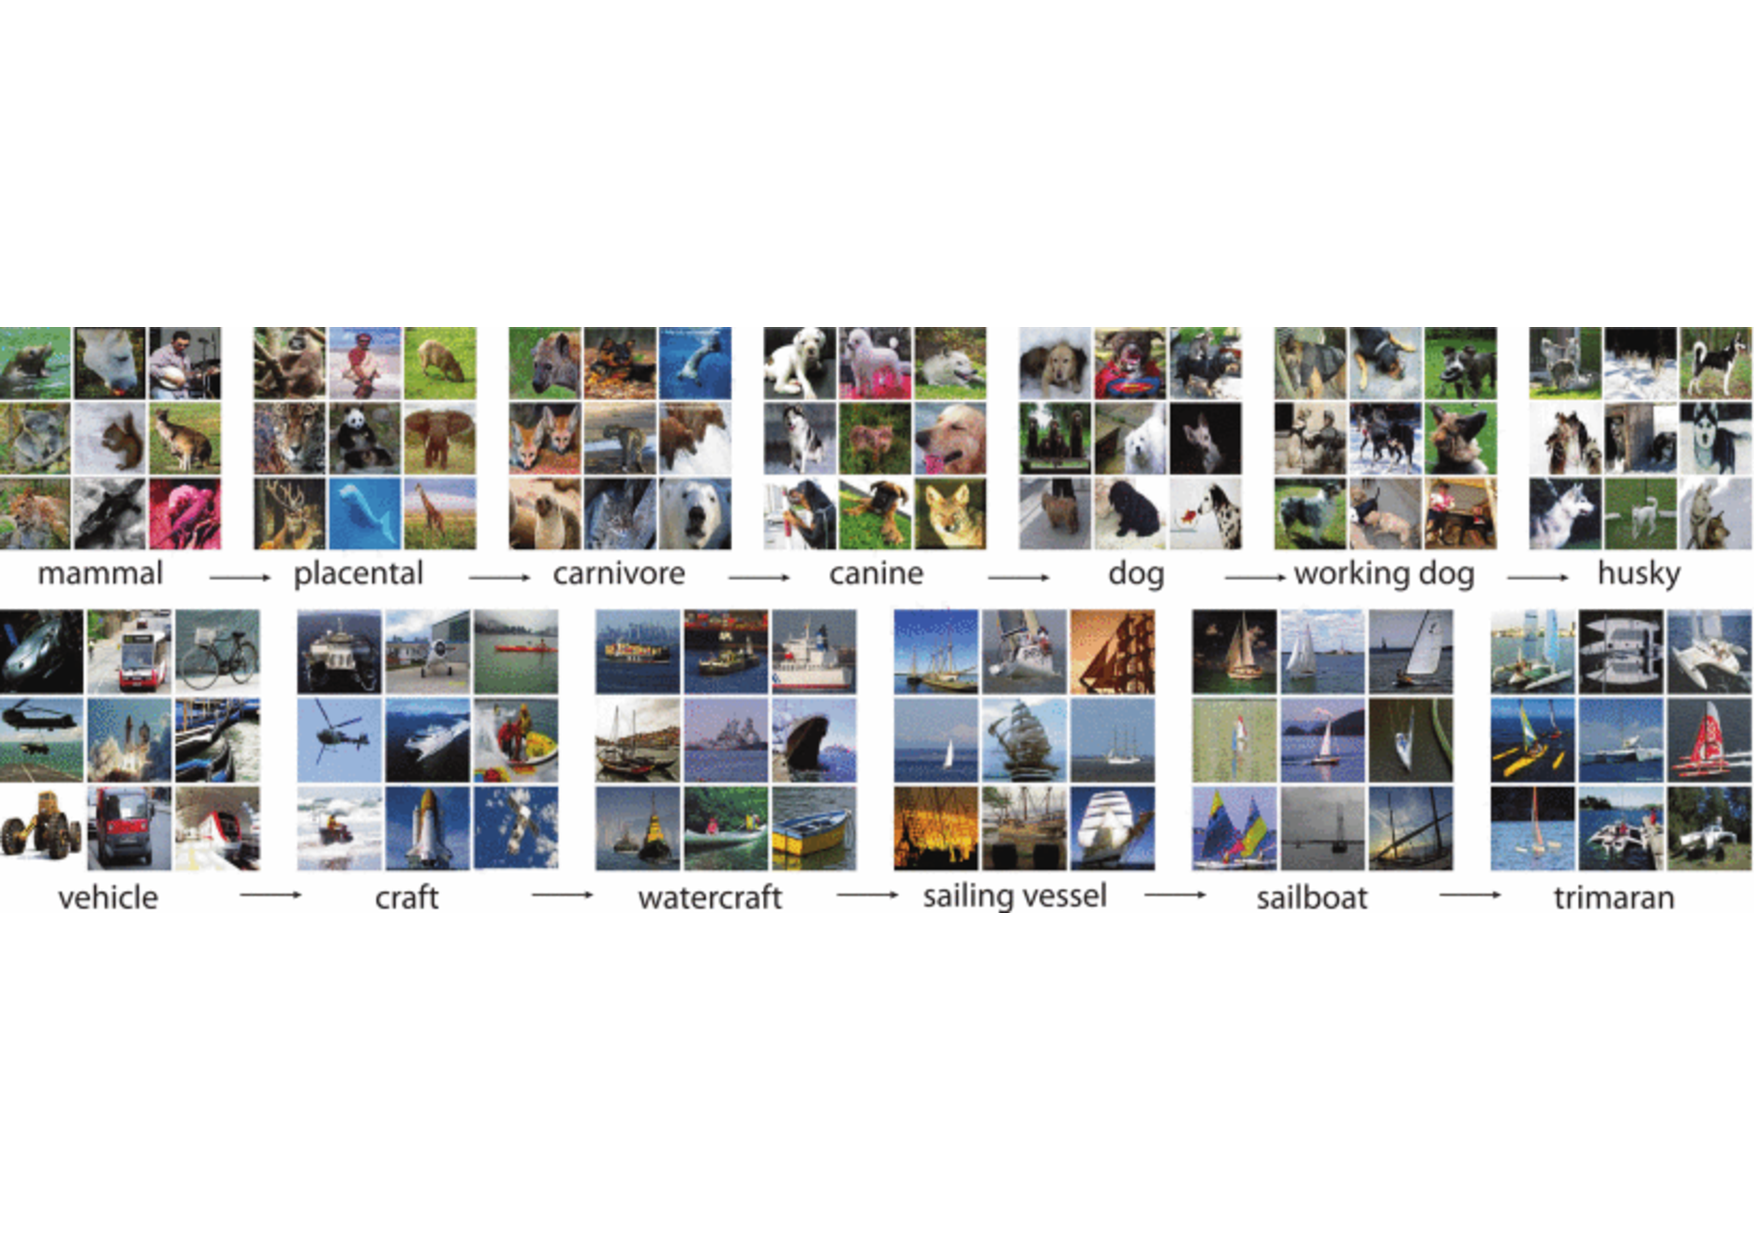
\includegraphics[width=0.9\textwidth]{./resources/images/Deng2009ImageNet_fig-1.pdf}
    \caption{Auszug aus dem ImageNet-Datensatz~\cite[Abb.~1]{Deng2009ImageNet}}
    \label{fig:imagenet}
  \end{figure}
\end{frame}

\begin{frame}{GTSRB}
  \begin{figure}
    \centering
    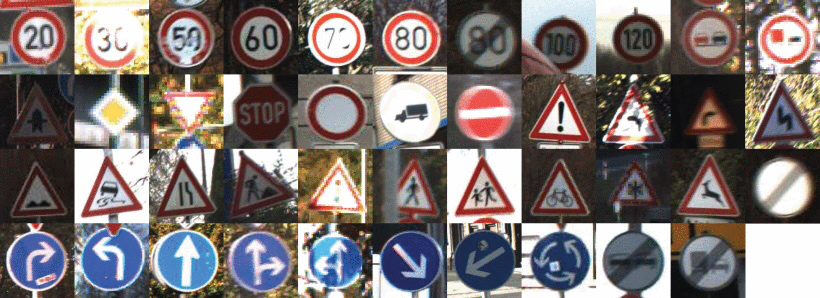
\includegraphics[width=0.9\textwidth]{./resources/images/gtsrb_classes.jpg}
    \caption{Auszug aus dem GTSRB-Datensatz~\cite[Abb.~3]{Stallkamp2011GTSRBCompetition}}
    \label{fig:gtsrb}
  \end{figure}
\end{frame}

\begin{frame}{Objekterkennung}
  \begin{itemize}
    \item Aber was ist mit Bildern, die mehrere~(verschiedene) Objekte enthalten?
    \item Oft ist auch die Position der Objekte wichtig
    \item[]
    \item<2-> Beispiel: Autonomes Fahren
    \item<2-> Zusätzlich zu den erkannten Objekten muss auch deren Position ermittelt werden
  \end{itemize}
\end{frame}

\begin{frame}{Bounding Boxen}\label{frame:bounding_box}
  \begin{itemize}
    \item Objekte im Bild werden durch Rechtecke~(Bounding Boxen) umschlossen
    \item Zwei weit verbreitete Formate
      \begin{enumerate}
        \item[]<2-> Bildecke oben links ist definiert als~(0, 0)\vspace{0.5cm}
        \item<3-> \(box = (box_x, box_y, box_w, box_h)\)
          \begin{itemize}
            \item \(box_x, box_y\): Mittelpunkt der Box
            \item \(box_w, box_h\): Breite und Höhe der Box
          \end{itemize}
        \item<4-> \(box = (box_{x1}, box_{y1}, box_{x2}, box_{y2})\)
          \begin{itemize}
            \item \(box_{x1}, box_{y1}\): Koordinaten der linken oberen Ecke
            \item \(box_{x2}, box_{y2}\): Koordinaten der rechten unteren Ecke
          \end{itemize}
      \end{enumerate}
  \end{itemize}
\end{frame}

\begin{frame}{Bounding Boxen}
  \begin{figure}
    \centering
    \includegraphics[width=0.9\textwidth]{./resources/images/Redmon2016YOLO_fig-6.pdf}
    \caption{Bounding Boxen in Bildern~\cite[Abb.~6]{Redmon2016YOLO}}
    \label{fig:bounding_box}
  \end{figure}
\end{frame}

\begin{frame}{Intersection over Union~(IoU)}
  \begin{columns}
    \begin{column}{0.6\textwidth}
      \begin{itemize}
        \item Wie gut ist eine Bounding Box?
        \item[]
        \item<2-> Intersection over Union~(IoU)
          \begin{itemize}
            \item \(IoU = \frac{A_{inter}}{A_{union}}\)
            \item \(A_{inter}\): Fläche der Überlappung
            \item \(A_{union}\): Fläche der Vereinigung
          \end{itemize}
        \item<2->[]
        \item<3-> IoU ist ein Maß für die Qualität der Bounding Box
          \begin{itemize}
            \item \(IoU = 1\): Box passt perfekt
            \item \(IoU = 0\): Box passt gar nicht
          \end{itemize}
      \end{itemize}
    \end{column}

    \begin{column}{0.4\textwidth}
      \begin{figure}
        \centering
        \only<2->{
          \includegraphics[width=0.9\textwidth]{./resources/images/Bishop2023Deep_fig-10_20.pdf}
          \caption{IoU~\cite[Abb.~10.20]{Bishop2023Deep}}
          \label{fig:iou_example}
        }
      \end{figure}
    \end{column}
  \end{columns}
\end{frame}

\begin{frame}[shrink=8]{Precision und Recall}
  \begin{columns}
    \begin{column}{0.4\textwidth}
      \begin{itemize}
        \item \(Precision = \frac{TP}{TP + FP}\)
        \item \(Recall = \frac{TP}{TP + FN}\)
        \item[]

          \only<2>{
          \item<2-3> \(TP\): True Positives
          \item \(FP\): False Positives
          \item \(FN\): False Negatives
          }
        \item<3->\textbf{Precision:}\\Wie viele der vorhergesagten Objekte sind tatsächlich vorhanden?\\\(\rightarrow\)~\enquote{Treffsicherheit}
        \item<4->\textbf{Recall:}\\Wie viele der tatsächlich vorhandenen Objekte wurden erkannt?\\\(\rightarrow\)~\enquote{Erfassungsrate}
      \end{itemize}
    \end{column}
    \begin{column}{0.6\textwidth}
      \begin{figure}
        \centering
        \only<2->{
          \resizebox{0.9\textwidth}{!}{\input{./resources/images/conf-matrix-tikz.tex}}
          \caption{Confusion Matrix}
          %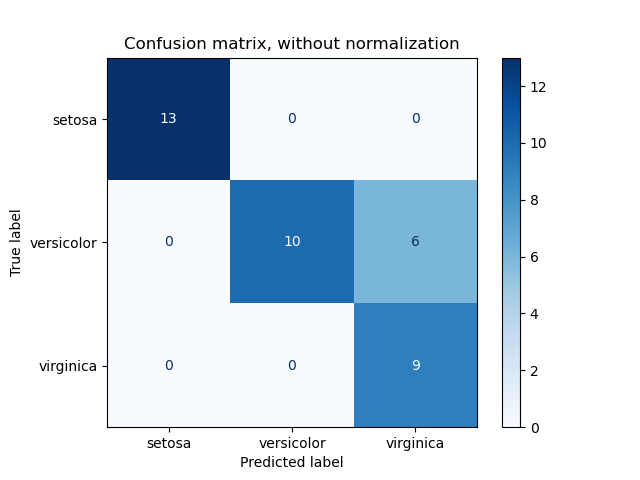
\includegraphics[width=0.9\textwidth]{./resources/images/Scikitlearn2025Confusion_confusion_matrix.png}
          %\caption{Confusion Matrix~\cite{Scikitlearn2025Confusion}}
          \label{fig:confusion_matrix}
        }
      \end{figure}
    \end{column}
  \end{columns}
\end{frame}

\begin{frame}{Mean Average Precision~(mAP)}
  \begin{columns}
    \begin{column}{0.6\textwidth}
      \begin{itemize}
        \item Wie gut ist ein Detektor?\\\cite{Everingham2010VOC,Lin2014COCO}
        \item[]
        \item<2-> Mean Average Precision~(mAP)
          \begin{itemize}
            \item \(mAP = \frac{1}{N} \sum_{i=1}^{N} AP_i\)
            \item \(AP_i\): Average Precision für Klasse~\(i\)
          \end{itemize}
        \item<2->[]
        \item<3-> Average Precision~(AP)
          \begin{itemize}
            \item \(AP_i = \int_0^1 P(r) dr\)
            \item \(P(r)\): Precision bei Recall~\(r\)
            \item In der Praxis: Fläche unter der Precision-Recall-Kurve
          \end{itemize}
      \end{itemize}
    \end{column}
    \begin{column}{0.4\textwidth}
      \begin{figure}
        \centering
        \only<3->{
          \resizebox{0.9\textwidth}{!}{\input{./resources/images/pr-curve-tikz.tex}}
          \caption{PR-Kurve}
          \label{fig:pr_curve}
        }
      \end{figure}
    \end{column}
  \end{columns}
\end{frame}

\begin{frame}{Regressionsausgabe}
  \begin{columns}
    \begin{column}{0.6\textwidth}
      \begin{itemize}
        \item OverFeat~\cite{Sermanet2013Overfeat} fügt den uns bereits bekannten CNNs eine zusätzliche Regressionsausgabe hinzu
        \item Diese vier Werte geben die Koordinaten der Bounding Box an~(siehe Folie~\ref{frame:bounding_box})
      \end{itemize}
    \end{column}
    \begin{column}{0.4\textwidth}
      \begin{figure}
        \centering
        \only<2->{
          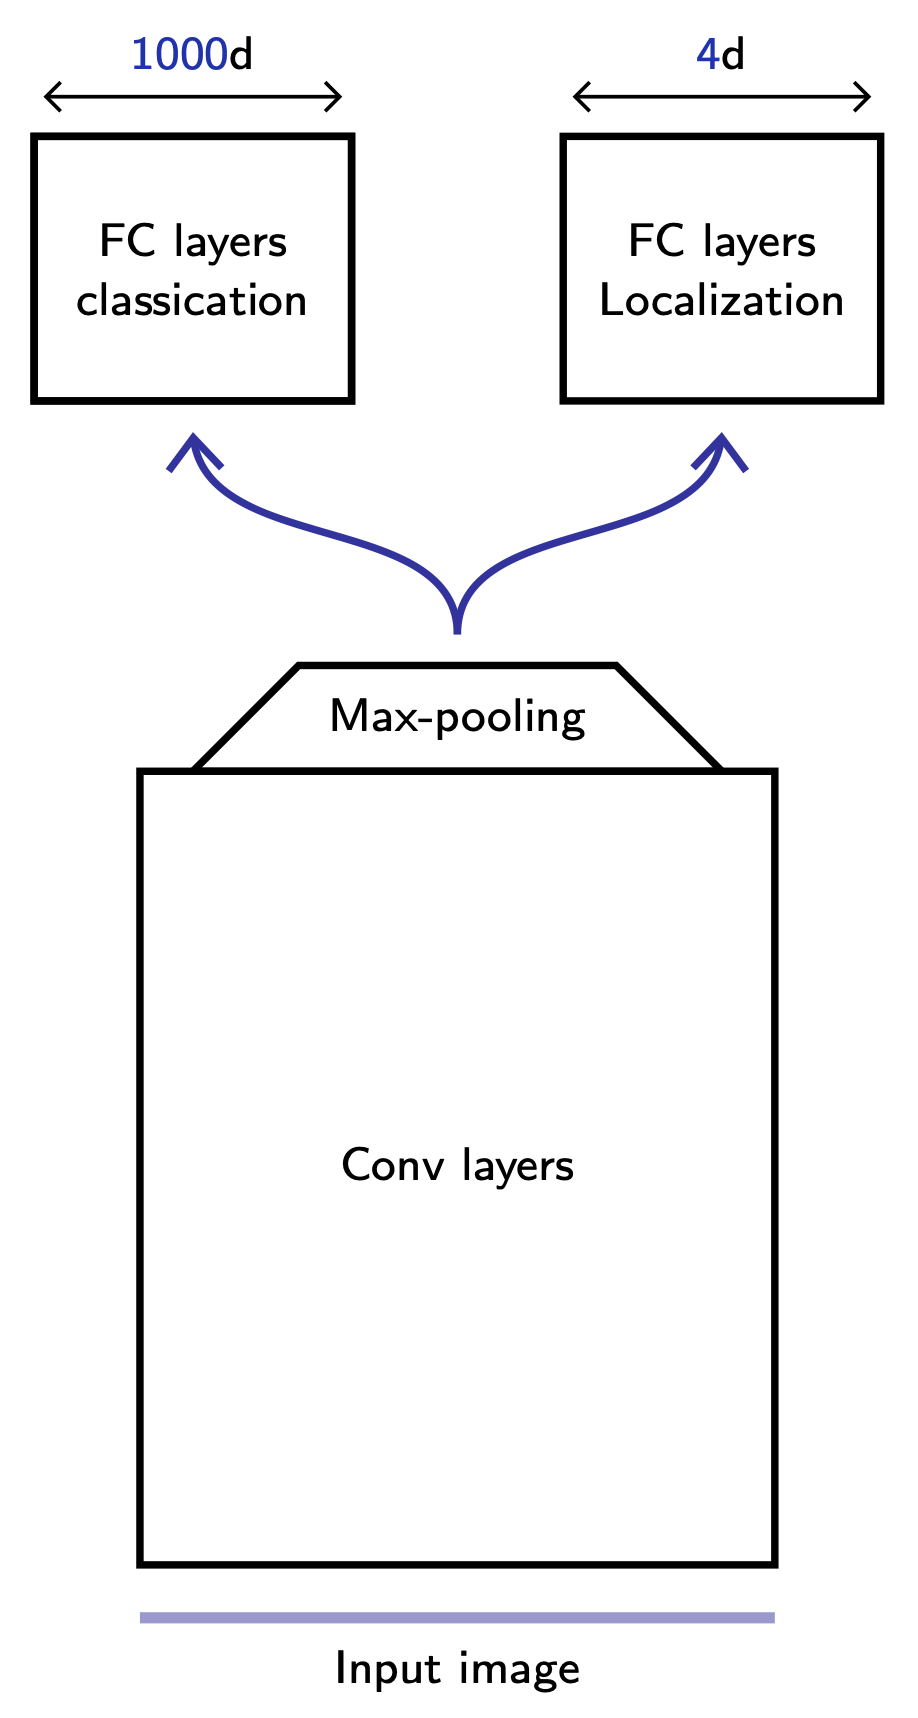
\includegraphics[width=0.6\textwidth]{./resources/images/Fleuret2022DLC_overfeat.png}
          \caption{Zusätzliche Regressionsausgabe~\cite[Kapitel~8.3.2]{Fleuret2022DLC}}
          \label{fig:regression_output}
        }
      \end{figure}
    \end{column}
  \end{columns}
\end{frame}

\begin{frame}{Sliding Windows}\label{frame:sliding_windows}
  \begin{itemize}
    \item Einfaches Verfahren zur Objekterkennung
    \item Ein Fenster wird schrittweise über das Bild geschoben
    \item Für jeden \enquote{Ausschnitt} des Bildes wird ein CNN aufgerufen\\\(\rightarrow\) Enthält dieser Ausschnitt ein Objekt?
    \item[]
    \item<2-> \textbf{Nachteil:} Unglaublich rechenintensiv
  \end{itemize}
\end{frame}

\begin{frame}{Region Proposals}
  \begin{itemize}
    \item Algorithmen, die Regionen im Bild vorschlagen, die Objekte enthalten könnten
    \item Geschieht anhand von Bildmerkmalen\\(z.\,B. Farben, Kanten, Texturen)
    \item Reduktion der Anzahl der CNN-Aufrufe im Vergleich zu Sliding Windows~(siehe Folie~\ref{frame:sliding_windows})
  \end{itemize}
\end{frame}

\begin{frame}{Zweistufige Objektdetektoren}
  \only<1-2>{
    \begin{enumerate}
      \item Regionen werden vorgeschlagen
      \item Regionen werden klassifiziert und Bounding Boxen werden berechnet
    \end{enumerate}
  }
  \begin{itemize}
    \item<2->[]
    \item<2-> Beispiele
      \begin{itemize}
        \item R-CNN~\cite{Girshick2014RCNN}
          \only<3>{
            \begin{itemize}
              \item Selective Search~\cite{Uijlings2013Selective} generiert Regionen
              \item Jede Region wird separat durch ein CNN verarbeitet
              \item Features werden separat für Klassifikation~(was ist es?) und Regression~(wo ist es?) verwendet
            \end{itemize}
          }
        \item Fast R-CNN~\cite{girshick2015FastRCNN}
          \only<4>{
            \begin{itemize}
              \item Feature-Sharing:~Das CNN verarbeitet das gesamte Bild nur einmal
              \item End-to-End-Training:~Zeitgleiches Training von Klassifikation und Regression
            \end{itemize}
          }
        \item Faster R-CNN~\cite{Ren2016FasterRCNN}
          \only<5>{
            \begin{itemize}
              \item Region Proposal Network~(RPN): Regionsvorschläge direkt aus den CNN-Features
              \item RPN teilt die CNN-Features mit dem Detektor
            \end{itemize}
          }
      \end{itemize}
  \end{itemize}
\end{frame}

\begin{frame}{Einstufige Objektdetektoren}
  \only<1-2>{
    \begin{itemize}
      \item Alles in einem Schritt
      \item Gesamtes Bild als Eingabe~(kein separater Region-Proposal-Schritt)
      \item Direkte Vorhersage der Bounding Boxen \textbf{und} Klassen
    \end{itemize}
  }
  \begin{itemize}
    \item<2->[]
    \item<2-> Beispiele
      \begin{itemize}
        \item YOLO~\cite{Redmon2016YOLO}
          \only<3>{
            \begin{itemize}
              \item Bild wird in ein \(S \times S\)-Gitter unterteilt
              \item Für jede Zelle werden Bounding Boxen~(\(B\)) und Klassenwahrscheinlichkeiten~(\(C\)) vorhergesagt
            \end{itemize}
          }
        \item SSD~\cite{Liu2016SSD}
          \only<4>{
            \begin{itemize}
              \item Fügt zusätzliche Faltungen~(Feature Maps) hinzu
              \item Ermöglicht einfachere Vorhersage von Objekten mit unterschiedlichen Größen
              \item Vorhersage der Bounding Boxen und Klassen auf mehreren Feature Maps
            \end{itemize}
          }
      \end{itemize}
  \end{itemize}
\end{frame}

\begin{frame}{YOLO}
  \begin{figure}
    \centering
    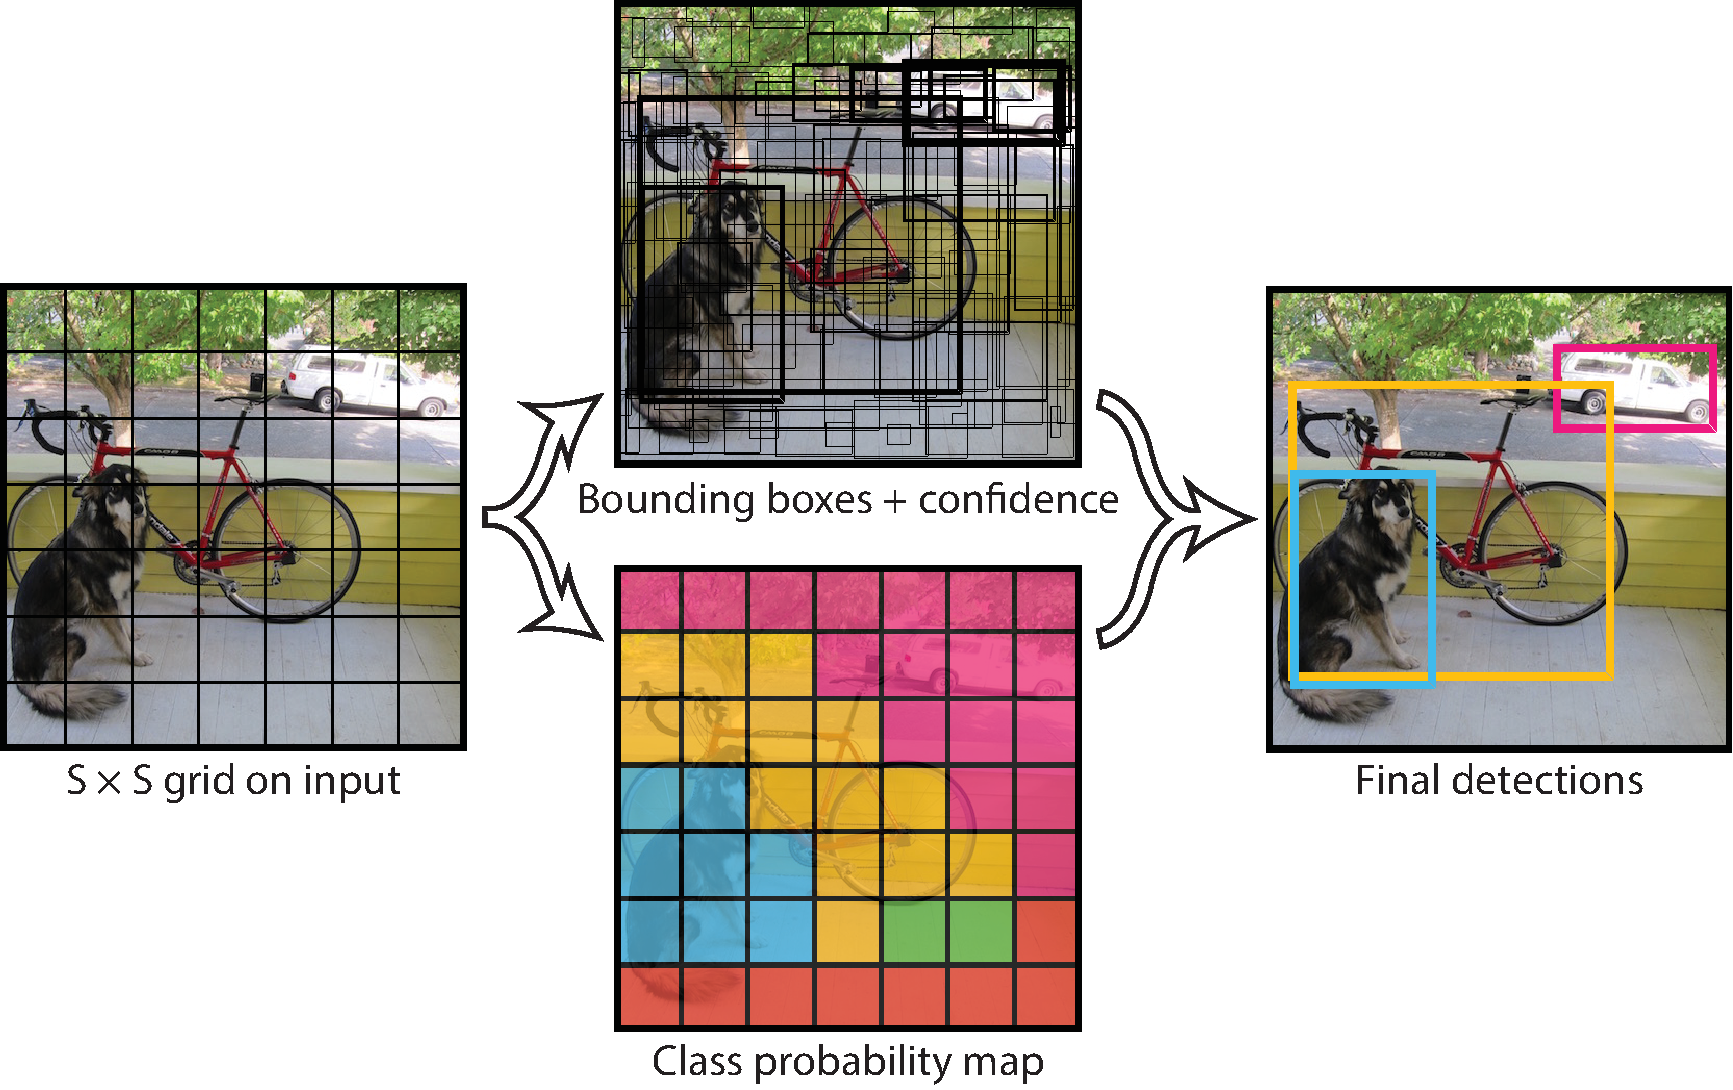
\includegraphics[width=0.9\textwidth]{./resources/images/Redmon2016YOLO_fig-2.pdf}
    \caption{YOLO-Modell, \(7 \times 7\)-Gitter~\cite[Abb.~2]{Redmon2016YOLO}}
    \label{fig:yolo_model}
  \end{figure}
\end{frame}

\begin{frame}{YOLO}
  \begin{figure}
    \centering
    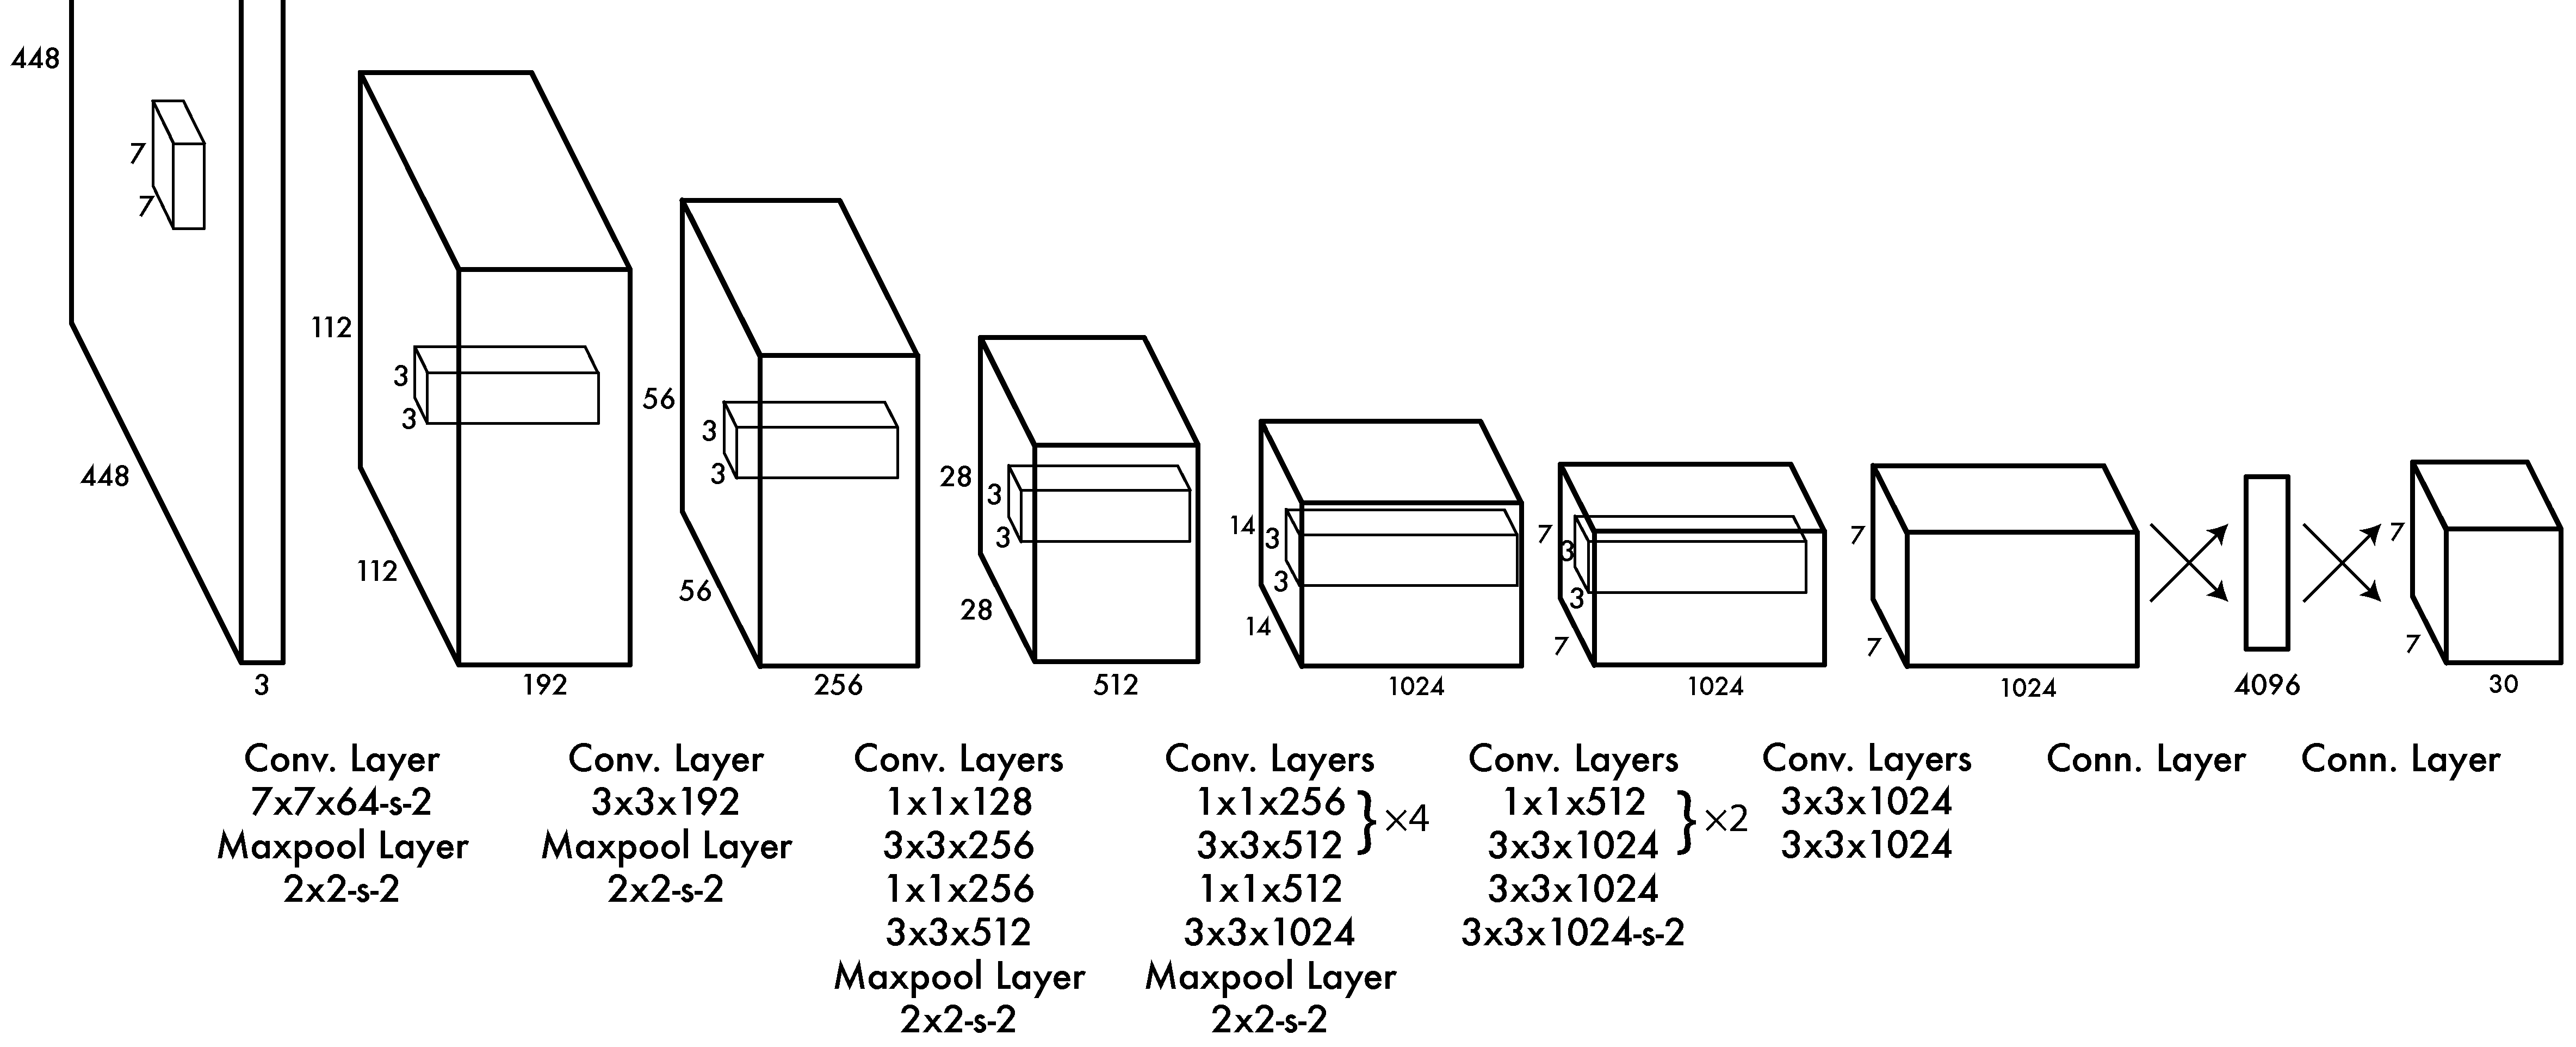
\includegraphics[width=0.9\textwidth]{./resources/images/Redmon2016YOLO_fig-3.pdf}
    \caption{YOLO-Architektur~\cite[Abb.~3]{Redmon2016YOLO}}
    \label{fig:yolo_architecture}
  \end{figure}
  \only<2->{
    \begin{itemize}
      \item Alle Komponenten sind uns bereits bekannt
        \begin{itemize}
          \item 24 Convolutional Layer
          \item 2 Fully Connected Layer
          \item Maxpooling Layers
          \item (Leaky) ReLU Aktivierungsfunktionen
          \item Output: \(S \times S \times (B \times 5 + C)\), hier mit \(S=7\), \(B=2\), \(C=20\)
        \end{itemize}
    \end{itemize}
  }
\end{frame}

\begin{frame}{YOLO}
  \begin{itemize}
    \item Stetige Weiterentwicklung
    \item YOLO/YOLOv1~(2016) -- YOLO12~(2025) -- YOLO26~(2026)
    \item[]
    \item<2-> Integration in eigene Projekte wird immer einfacher~\cite{Ultralytics2026Yolo}
      \begin{itemize}
        \item \texttt{pip install ultralytics}
        \item \texttt{from ultralytics import YOLO}
        \item \texttt{model = YOLO("yolo26n.pt")}
        \item \texttt{results = model.predict(source="video.mp4")}
        \item \texttt{results[0].plot()}
      \end{itemize}
  \end{itemize}
\end{frame}

\begin{frame}{Zusammenfassung}
  \begin{itemize}
    \item<1-> Objekterkennung als wichtiges Anwendungsgebiet von CNNs
    \item<2-> Unterscheidung zwischen
      \begin{itemize}
        \item Zweistufige Detektoren~(z.\,B.~R-CNN, Fast R-CNN, Faster R-CNN)
        \item Einstufige Detektoren~(z.\,B.~\textbf{YOLO}, SSD)
      \end{itemize}
    \item<3-> Grundsätzlich sind zweistufige Detektoren genauer und einstufige Detektoren schneller
    \item<4-> YOLO ist so beliebt, weil Echtzeit-Objekterkennung ein spannendes Anwendungsgebiet ist
  \end{itemize}
\end{frame}

\begin{frame}{Ausblick}
  \begin{itemize}
    \item Bildsegmentierung
    \item Transformer-basierte Detektoren~(z.\,B.~DETR~\cite{Carion2020End})
  \end{itemize}
\end{frame}

\begin{frame}[allowframebreaks, noframenumbering, plain]{Quellen}
  \sloppy
  \printbibliography
\end{frame}

\end{document}
